\documentclass{article}

% this part goes in the preamble

\def \setA{ (0, 0) circle (1cm) }
\def \setB{ (1.5, 0) circle (1cm) }
\def \setC{ (0.75, 1) circle (1cm) }

\def \colorA{red}
\def \colorB{blue}
\def \colorC{white}
\def \colorAB{purple}
\def \colorAC{red}
\def \colorBC{blue}
\def \colorABC{purple}
\usepackage{tikz}
\usetikzlibrary{shapes, backgrounds}

\begin{document}
% this part goes where you want the figure!
\begin{center}
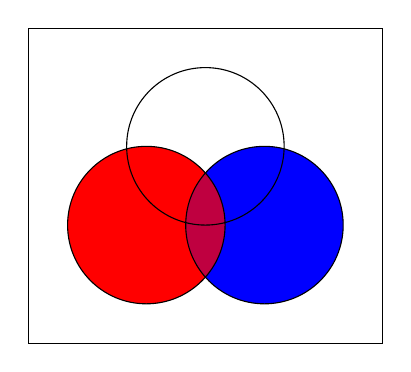
\begin{tikzpicture}
\fill[\colorA] \setA;
\fill[\colorB] \setB;
\fill[\colorC] \setC;
\begin{scope}
 \clip \setA;
 \fill[\colorAB] \setB;
 \end{scope}
\begin{scope}
 \clip \setA;
 \fill[\colorAC] \setC;
 \end{scope}
\begin{scope}
 \clip \setB;
 \fill[\colorBC] \setC;
 \end{scope}
\begin{scope}
 \clip \setA;
 \clip \setB;
 \fill[\colorABC] \setC;
\end{scope}

\draw \setA;
\draw \setB;
\draw \setC;
\draw (-1.5, -1.5) rectangle (3, 2.5);
\end{tikzpicture}
\end{center}

\end{document}
